\documentclass[twoside]{article}
\usepackage{../../estilo-ejercicios}
\newcommand{\colapso}{{\searrow\!\!\!\!\searrow}}
%--------------------------------------------------------
\begin{document}

\title{Ejercicios de Homología Simplicial}
\author{Diego Pedraza López, Javier Aguilar Martín}
\maketitle

\begin{ejercicio}{2.1}
Probar que si $K$ es un complejo simplicial conexo, entonces
$\Im[∂_1 : C_1(K; \F) → C_0(K; \F)]$ es el subespacio de todas las cadenas $∑λ_iv_i$ con $∑λ_i = 0$.
Deducir que $H_0(K; \F) \cong \F$ generado por la clase de homología de cualquier vértice de $K$.
\end{ejercicio}
\begin{solucion}

\end{solucion}

\newpage

\begin{ejercicio}{2.2}
Probar que $\widetilde{H}_0(K; \F) = \ker[c_∗ : H_0(K; \F) → H_0(\{v\}; \F)]$ donde $c : K →
\{v\}$ es la aplicación constante. Deducir $H_0(K; \F) \cong \widetilde{H}_0(K; \F)
⊕F$.
\end{ejercicio}
\begin{solucion}

\end{solucion}

\begin{solucion}
\end{solucion}


\newpage

\begin{ejercicio}{2.3}
Probar que si $K_1, \dots , K_s$ son las componentes conexas de $K$, entonces
para cualquier $p ≥ 0$, $H_p(K; \F) \cong
⊕^s_{i=1}
H_p(K_i; \F)$, siendo los generadores de $H_0(K; \F)$ las
clases de homología de un vértice cualquiera por cada componente
\end{ejercicio}
\begin{solucion}

\end{solucion}

\newpage

\begin{ejercicio}{2.4}
Dar un ejemplo de dos complejos simpliciales no simplicialmente isomorfos
pero que tengan sus homologías isomorfas.
\end{ejercicio}
\begin{solucion}
$\{v_0,v_1,v_2,v_3,(v_0,v_1),(v_0,v_2), (v_0,v_3), (v_1,v_2)\}$ y $\{v_0,v_1,v_2,(v_0,v_1),(v_0,v_2), (v_1,v_2)\}$.
\end{solucion}

\newpage

\begin{ejercicio}{2.5}
Probar que para todo $p ≥ 0$, se tiene
\[
C_p(K; \F) \cong Z_p(K; \F)
⊕B_{p−1}(K; \F)
\]
y deducir
\[
C_p(K; \F)/B_p(K; \F) \cong H_p(K; \F)
⊕B_{p−1}(K; \F).
\]
\end{ejercicio}
\begin{solucion}


\end{solucion}

\newpage

\begin{ejercicio}{2.6}
Sea $K$ un complejo simplicial y $K^m$ su $m$-esqueleto. Probar que $H^n(K; \F) =
H^n(K^m; \F)$ si $n < m$. ¿Qué relación hay entre $H^m(K; \F)$ y $H^m(K^m; \F)$?

\end{ejercicio}
\begin{solucion}

\end{solucion}

\newpage

\begin{ejercicio}{2.7}
Dado un complejo simplicial $K$, probar que $H_n(ΣK) \cong H_{n−1}(K)$ para
todo $n ≥ 0$.

\end{ejercicio}
\begin{solucion}

\end{solucion}

\newpage

\begin{ejercicio}{2.8}
Sea $G$ un grafo orientado y $e_1, \dots , e_µ$ aristas tales que $T = G−\{e_1, \dots , e_µ\}$
es un árbol maximal. Se denotará por $T+e_i$ al grafo $T∪\{e_i\}$. Dicho grafo contiene un único
lazo $l_i$, al cual se le puede asociar un 1-ciclo $z_i$, formado por las aristas de $l_i$ con coeficientes
$±1$, segúnn la orientación inducida por el recorrido de $l_i$ coincida con la orientación asignada
en $z_i$ para que $e_i$ aparezca con coeficiente $+1$. Prueba que $\{z_1, \dots , z_µ\}$ es una base para
$H_1(G; \F)$. Es decir, $H_1(G; \F) \cong ⊕_{µ(G)}\F$. Deduce que si $G$ es conexo con $µ(G) = 1$ entonces
$G$ tiene un único lazo.
\end{ejercicio}
\begin{solucion}

\end{solucion}

\newpage

\begin{ejercicio}{2.9}
Calcular los F-espacios vectoriales de homología de $K$, siendo $K =
\partial^n
∨
\partial σ^m$
\end{ejercicio}
\begin{solucion}

\end{solucion}

\newpage

\begin{ejercicio}{2.10}
Obtener los $\F$-espacios vectoriales de homología del complejo abstracto
$C$ correspondiente a la triangulación del cilindro vista en clase.
\end{ejercicio}
\begin{solucion}

\end{solucion}

\newpage

\begin{ejercicio}{2.11}
Calcular los $\F$-espacios vectoriales de homologíaa del complejo abstracto
$M$ correspondiente a la triangulación de la banda de Möbius vista en clase.
\end{ejercicio}
\begin{solucion}
\end{solucion}

\newpage

\begin{ejercicio}{2.12}
Demostrar que la homología simplicial (reducida) con coeficientes en
cualquier cuerpo $\F$ de la triangulación del sombrero bobo vista en clase es trivial. Sin
embargo, comprobar que $L$ no es colapsable.
\end{ejercicio}
\begin{solucion}


$L$ no es colapsable porque no tiene caras libres
\end{solucion}

\newpage

\begin{ejercicio}{2.13}
Sea $σ$ un $n$-símplice y $K$ el complejo formado por $σ$ y sus caras. Probar
que si $0 < q < n$, $H_q(K^q
; \F)$ es un $\F$-espacio vectorial de dimensión $\binom{n}
{q+1}$.
\end{ejercicio}
\begin{solucion}

\end{solucion}

\newpage

\begin{ejercicio}{2.14}
Calcular los $\F$-espacios vectoriales de homología de $K$, siendo $K$ la triangulación
del toro con una membrana vista en clase.
\end{ejercicio}
\begin{solucion}

\end{solucion}

\newpage

\begin{ejercicio}{2.15}
Triangular el espacio $X ⊆ \R^2$
consistente en $k$ circunferencias disjuntas
$S_1, \dots , S_k$ y un segmento $A$ tangente a cada una de ellas y calcular sus $\F$-espacios
vectoriales de homología.
\end{ejercicio}
\begin{solucion}

\end{solucion}

\newpage

\begin{ejercicio}{2.16}
Dados los conjuntos de $\R
^3$
\[
A = \{(x, y, z); x^2 + y^2 + z^2 = 1, x ≤ 0\}\]
\[
B = \{(x, y, z) ∈ \R^3
; x^2 + y^2 + z^2 = 1, x ≥ 0, z = 0\}
\]
sea $X = A
∪
B$. Triangular el espacio $X$ y hallar los $\F$-espacios vectoriales de homología
correspondientes a dicha triangulación.
\end{ejercicio}
\begin{solucion}

\end{solucion}

\newpage

\begin{ejercicio}{2.17}
Dado el espacio $Y = A
∪
B$, donde
\[
A = \{(x, y, z) ∈ \R^3
; x^2 + y^2 + z^2 = 1\}
\]
\[
B = \{(x, y, z) ∈ \R^3
; x = 0, z = 0, −1 ≤ y ≤ 1\}
\]
triangular $Y$ y hallar los $\F$-espacios vectoriales de homología correspondientes a esa triangulación
\end{ejercicio}
\begin{solucion}
 
\end{solucion}

\newpage

\begin{ejercicio}{2.18}
Sea $X$ el subespacio de $\R^3$
consistente en una esfera encajada por
su ecuador en un toro. Triangular $X$ y calcular los $\F$-espacios vectoriales de homología
simplicial de $X$. Determinar también la carcaterística de Euler-Poincaré $χ(K)$.
\end{ejercicio}
\begin{solucion}
\end{solucion}

\newpage

\begin{ejercicio}{2.19}
Calcular los $\F$-espacios vectoriales de homología de un cilindro con dos
agujeros.
\end{ejercicio}
\begin{solucion}
\end{solucion}

\newpage

\begin{ejercicio}{2.20}
Calcular los $\F$-espacios vectoriales de homología de:

\begin{figure}[h!]
\centering
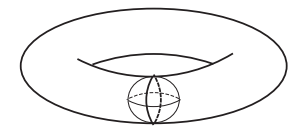
\includegraphics[scale=0.7]{toro1}
\end{figure}
\end{ejercicio}
\begin{solucion}
\end{solucion}

\newpage

\begin{ejercicio}{2.21}
Calcular los $\F$-espacios vectoriales de homología de dos toros entrelazados:

\begin{figure}[h!]
\centering
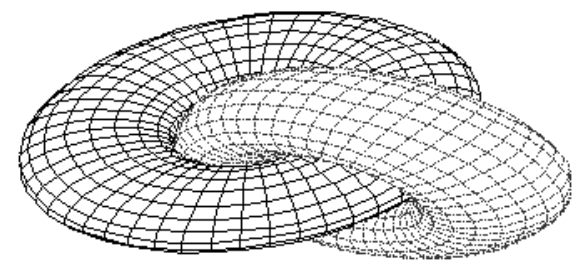
\includegraphics[scale=0.5]{toro2}
\end{figure}
\end{ejercicio}

\begin{solucion}
\end{solucion}

\newpage

\begin{ejercicio}{2.22}
Probar que los espacios euclídeos $\R^n$
y $\R^m$ no son homeomorfos si $n\neq m$.
\end{ejercicio}
\begin{solucion}
\end{solucion}
\newpage

\begin{ejercicio}{2.23}
Dar un ejemplo de dos espacios topológicos no homeomorfos pero que
tengan todos sus $\F$-espacios vectoriales de homología isomorfos.
\end{ejercicio}
\begin{solucion}
Considerar las realizaciones geométricas de los complejos del ejercicio \ref{ejer:2.4}.
\end{solucion}

\end{document}
